\begin{algorithm}[!t]
\small
\caption{Label propagation algorithm}
\label{alg:SV_ALG}
\begin{algorithmic}[1]
\Require {$G=(V,E)$}

\State Initialization ;
\For {each $v\in V$}
\State	$CC[v]=v; CCp[v]=v$;
\EndFor

\State $NumChange=|V|$
\While{$NumChange>0$};
\State $NumChange\leftarrow 0$
\State MemCpy($CCp$,$CC$,$|V|$)
\For {each $v\in V$}
\For {each $u\in E(v)$}

\If {$CCp[u]<CC[v]$}
\State $CC[v]\leftarrow CCp[u]$
\State NumChanges = NumChanges+1;
\EndIf

\EndFor
\EndFor

\EndWhile 


\end{algorithmic}
\end{algorithm}
%
Given a undirected Graph $G=(V,\ E)$, a connected-component $C$ is a subset of
vertex $V$ which satisfies the following.  A) there is a path between any two
vertices of $C$ in the parent graph $G$;  and B) there are no paths between
any vertex in $C$ and $V-C$. We would like to find all the connected
components in a graph. This problem is known as graph connected component
problem.

 We focus on the highly parallel label-propagation algorithm for the graph
connected-component problem.  We describe the working of label propagation
algorithm relevant to our discussion later. \paragraph{Label Propagation
algorithm in Fault Free execution}

\begin{figure*}

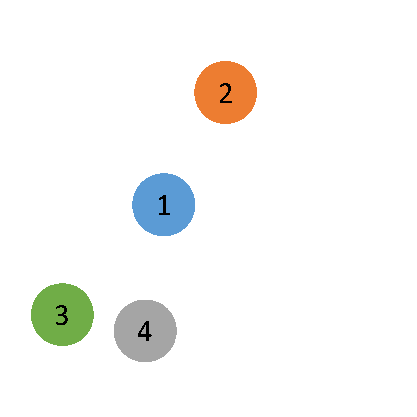
\includegraphics[width=0.2\textwidth]{figure/sv1}
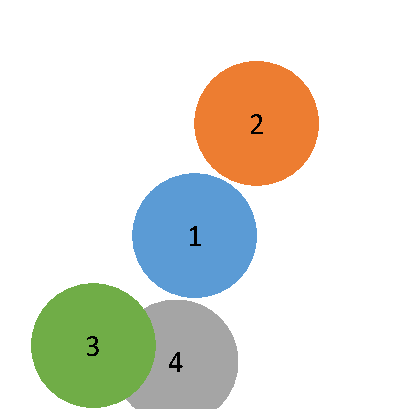
\includegraphics[width=0.2\textwidth]{figure/sv2}
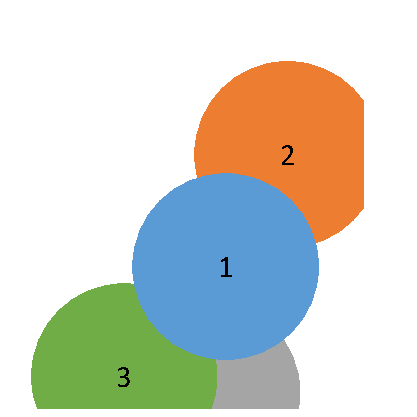
\includegraphics[width=0.2\textwidth]{figure/sv3}
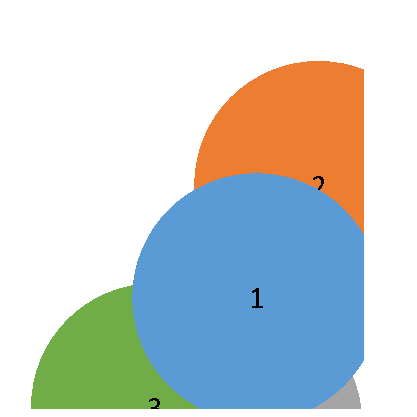
\includegraphics[width=0.2\textwidth]{figure/sv4}
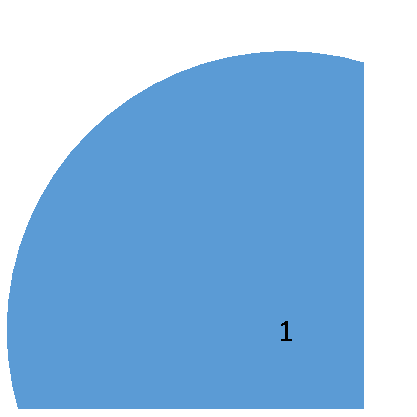
\includegraphics[width=0.2\textwidth]{figure/sv5}
\caption{
\label{fig:svalgm}
These sub-figures conceptually show how the connected component id
propagates through the graph as time evolves. Subfigures represent
snapshots of the algorithm at different times. For simplicity, this
example assumes that all the shown vertices are connected. Initially
the number of connected components is equal to the number vertices.
(a) Depicts the initial state in which each vertex is in its own component.
(b)-(d) depict that some vertices belong to the same connected component
yet may require multiple label updates (in either the same iteration
or a separate iteration). (e) is the final state in which there is
a single connected component.}

\end{figure*}

\begin{table}

\centering
\footnotesize
\caption{Symbols used in the fault free \sv algorithm and in the new fault tolerant algorithm.}
\begin{tabular}[t]{|l|l|r|}\hline
Symbol & Decription & Size\\\hline\hline
$V$ & Vertices in the graph & O(V)\\\hline
$E$ & Edges in the graph & O(E)\\\hline
$adj(v)$ & Adjacency list for vertex $v\in V$ & \\\hline
\CCVAL & Connected component array & O(V)\\\hline
\CCVAL$^i$ & Connected component array after iteration $i$ & O(V)\\\hline
\CCVAL$^\infty$ & The final connected component mapping upon algorithm completion. & O(V)\\\hline

& Fault free \\
\hline
$H$ &  & O(V)\\\hline
\end{tabular}
\label{tab:symbols}

\end{table}

The label propagation algorithm marks each vertex with a label that identifies
its component. The identifying label can be the minimum vertex-id in the
component. The label-marking process is iterative. In every iteration, each
vertex computes the minimum label amongst itself and its neighbors. So the
minimum label propagates to all the vertex in the component. The algorithm
stops when every vertex in the graph has acquired its final label.

The label propagation algorithm keeps an array $CC$ of current labels of all
vertices. For each vertex $v$, its label $CC[v]$ is initialized with its
vertex-id $CC[v]=v$. In every iteration, each vertex updates its label by
calculating minimum label of all its neighbors and itself: 
%
\begin{equation}
CC^{i+1}[v]=\min_{u\in\mathcal{N}(v)}CC^{i}[u],\label{eq:lp_update_eqn}
\end{equation}

Where $\mathcal{N}(v)=\left\{ v,adj(v)\right\} $ is the defined as immediate
neighbourhood of $v$. So the minimum vertex-id propagates to all the vertices
in the connected component. The iteration converges when there are no more
label changes in the graph. We show the pseudo-code for label propagation algorithm in \cref{alg:SV_ALG}.
In \cref{alg:SV_ALG}, we also update the \emph{parent} array $P[v]$, which
tracks the vertex which causes the last change  in the label  of $v$. 

We can implement \cref{eq:lp_update_eqn} can in two ways. In a first way, we
use two different arrays to store $CC^{i+1}$ and $CC^{i}$. We refer to this
implementation is \synclp~algorithm. In another way, we overwrite $CC^{i+1}$
on $CC^{i}$. We refer to this version as \asynclp~algorithm. Depending on
architecture and programming model, the two variants may have different
performance characteristics. In the subsequent discussion, we assume
\asynclp~algorithm. Yet, our results are equally applicable to both instances
of the \sv algorithm.

\textbf{\emph{ Cost of Label-propagation Algorithm: }}
Each iteration of \sv, we visit all the vertex and edges once and thus
costs $\mathcal{O}(V+E)$. The LP algorithm requires $\mathcal{O}(d)$
iterations to converge, where $d$ is the diameter of the graph. We
may use short-cutting to bound the number of iteration to $\mathcal{O}(log(d))$
{[}insert citation{]}. However, in practice \asynclp algorithm only
takes a few more iteration than implementing full short cutting step,
without the cost of short cutting. 
